\begin{flushleft}
\textbf{\LARGE{\textsc{Collapse Algorithm}}} \\
\textbf{\large{Ronald J. Botelho, MS}} \\
\textbf{\normalsize{Binghamton University, School of Systems Science}} \\
\textbf{\normalsize{2025}} \\
\end{flushleft}

\newpage

\section*{Epigraph}
\begin{quote}
\textit{``The most effective way to destroy people is to deny and obliterate their own understanding of their history.''} \\
\hfill --- George Orwell
\end{quote}

\vspace{1cm}

\begin{quote}
\textit{``Any logically irreversible manipulation of information, such as the erasure of a bit or the merging of two computation paths, must be accompanied by a corresponding entropy increase in non-information-bearing degrees of freedom of the information-processing apparatus or its environment.''} \\
\hfill --- Rolf Landauer (1961)
\end{quote}

\newpage

\section*{Abstract}
This book investigates the engineered collapse of democratic norms in the United States through a systems science lens. It draws on interdisciplinary methods to examine the weaponization of information, institutional decay, judicial permissiveness, and economic coercion. From media disinformation campaigns to Supreme Court rulings that hollow out civil liberties, the Collapse Algorithm charts how interconnected mechanisms feed systemic regression.

Across fifteen chapters, the work constructs a feedback model of collapse, grounded in entropy theory, power consolidation, and memory suppression. It concludes by proposing countervailing strategies rooted in resistance, transparency, and the rekindling of civic memory.

\newpage

\section*{Preface}
This book began as an act of warning and became an act of preservation. When I first noticed the structural echoes between modern America and other collapsed regimes I had studied, I felt compelled to document the parallels. What began as observation soon became diagnosis. What became diagnosis evolved into resistance.

These chapters are drawn from both lived experience and scholarly interrogation. I owe much to the professors who challenged my assumptions, the classmates who offered brutal honesty, and the voices—past and present—who refused to forget.

Every word here is written in defiance of the systems that would rather you forget. It is an offering of memory, a cartography of collapse, and a blueprint for survival.

\begin{flushright}
\textit{--- Ronald J. Botelho, 2025}
\end{flushright}

\newpage

\section*{Prologue: Entropy in the System}
In the quiet spaces between headlines, systems erode. Not with explosions, but with entropy—measured, incremental loss. The second law of thermodynamics tells us that in every closed system, disorder increases. So too does it unfold in democracy.

The feedback loop that hastens collapse is not merely metaphorical. It is thermodynamic. Shannon’s information theory taught us that uncertainty—or entropy—rises as messages become noisy. Landauer’s principle added that information loss has an energy cost. When history is erased, when disinformation corrupts, the system doesn’t just forget—it degrades.

This book frames collapse through that scientific lens. Language becomes code. Governance becomes entropy. Every suppression of truth introduces heat into the system—distortions that, if left unchecked, evolve into breakdown.

In these pages, we analyze America’s ongoing unraveling through the lens of entropy, compression, and coercion. From Supreme Court reversals to AI-driven propaganda, the mechanisms of collapse are traced with precision. You’ll see graphs, models, and third-order Markov matrices. But beneath it all is a human cry: memory is being murdered.

The algorithm is not simply computational. It is political. It is judicial. It is cultural. It is collapsing.

\begin{flushright}
\textit{Let us chart it, before the last bit fades.}
\end{flushright}

\newpage

\chapter{Privatized Memory and the Corporate State}

\section*{Introduction}
The erosion of democratic infrastructure is no longer confined to state institutions. In an alarming acceleration of neoliberal doctrine, private entities have been granted unprecedented access to sensitive governmental operations. The recent June 2025 Supreme Court ruling, granting the Trump administration legal cover to share sensitive information with private contractors such as Palantir Technologies, has redefined the contours of civic power, accountability, and memory (Supreme Court of the United States, 2025).

\section{The Gaslighting Infrastructure of Privatized Surveillance}
Palantir’s systems have become synonymous with algorithmic surveillance, predictive policing, and undocumented database aggregation. Yet, what is most insidious is their role in narrative construction. Through their proprietary algorithms—black boxes beyond public audit—Palantir shapes how agencies see threats, immigrants, protestors, and dissenters. Their software is not merely informational; it is epistemological. It decides what is known, what is emphasized, and what is ignored.

The Supreme Court’s majority opinion has now sanctioned a form of judicial outsourcing. Epistemic sovereignty—the right to determine what is true within the public record—has been transferred to a private actor with clear ideological alignments and commercial motives.

\section{Thermodynamic Implications: Erasure with a Cost}
Using our adapted entropy model, we calculate the Landauer cost of each institutional erasure event linked to Palantir’s involvement. Each undocumented data purge, each unacknowledged detainment justified by predictive flags, and each court decision that avoids precedent accrues thermodynamic debt. The system overheats—legally, politically, and morally.

\section{Narrative Drift Visualization (TPM)}
A third-order Markov transition probability matrix (TPM) was constructed based on a corpus of DHS and ICE internal policy changes from 2015–2025. The visualization, titled "Drip Map of Authoritarian Drift," demonstrates:

\begin{itemize}
  \item High entropy migration from constitutional norms to authoritarian practices.
  \item Compression of civic language and public transparency post-2020.
  \item Sharp KL divergence between pre-2016 DHS lexicon and post-2023 enforcement narratives.
\end{itemize}

\begin{figure}[h!]
  \centering
  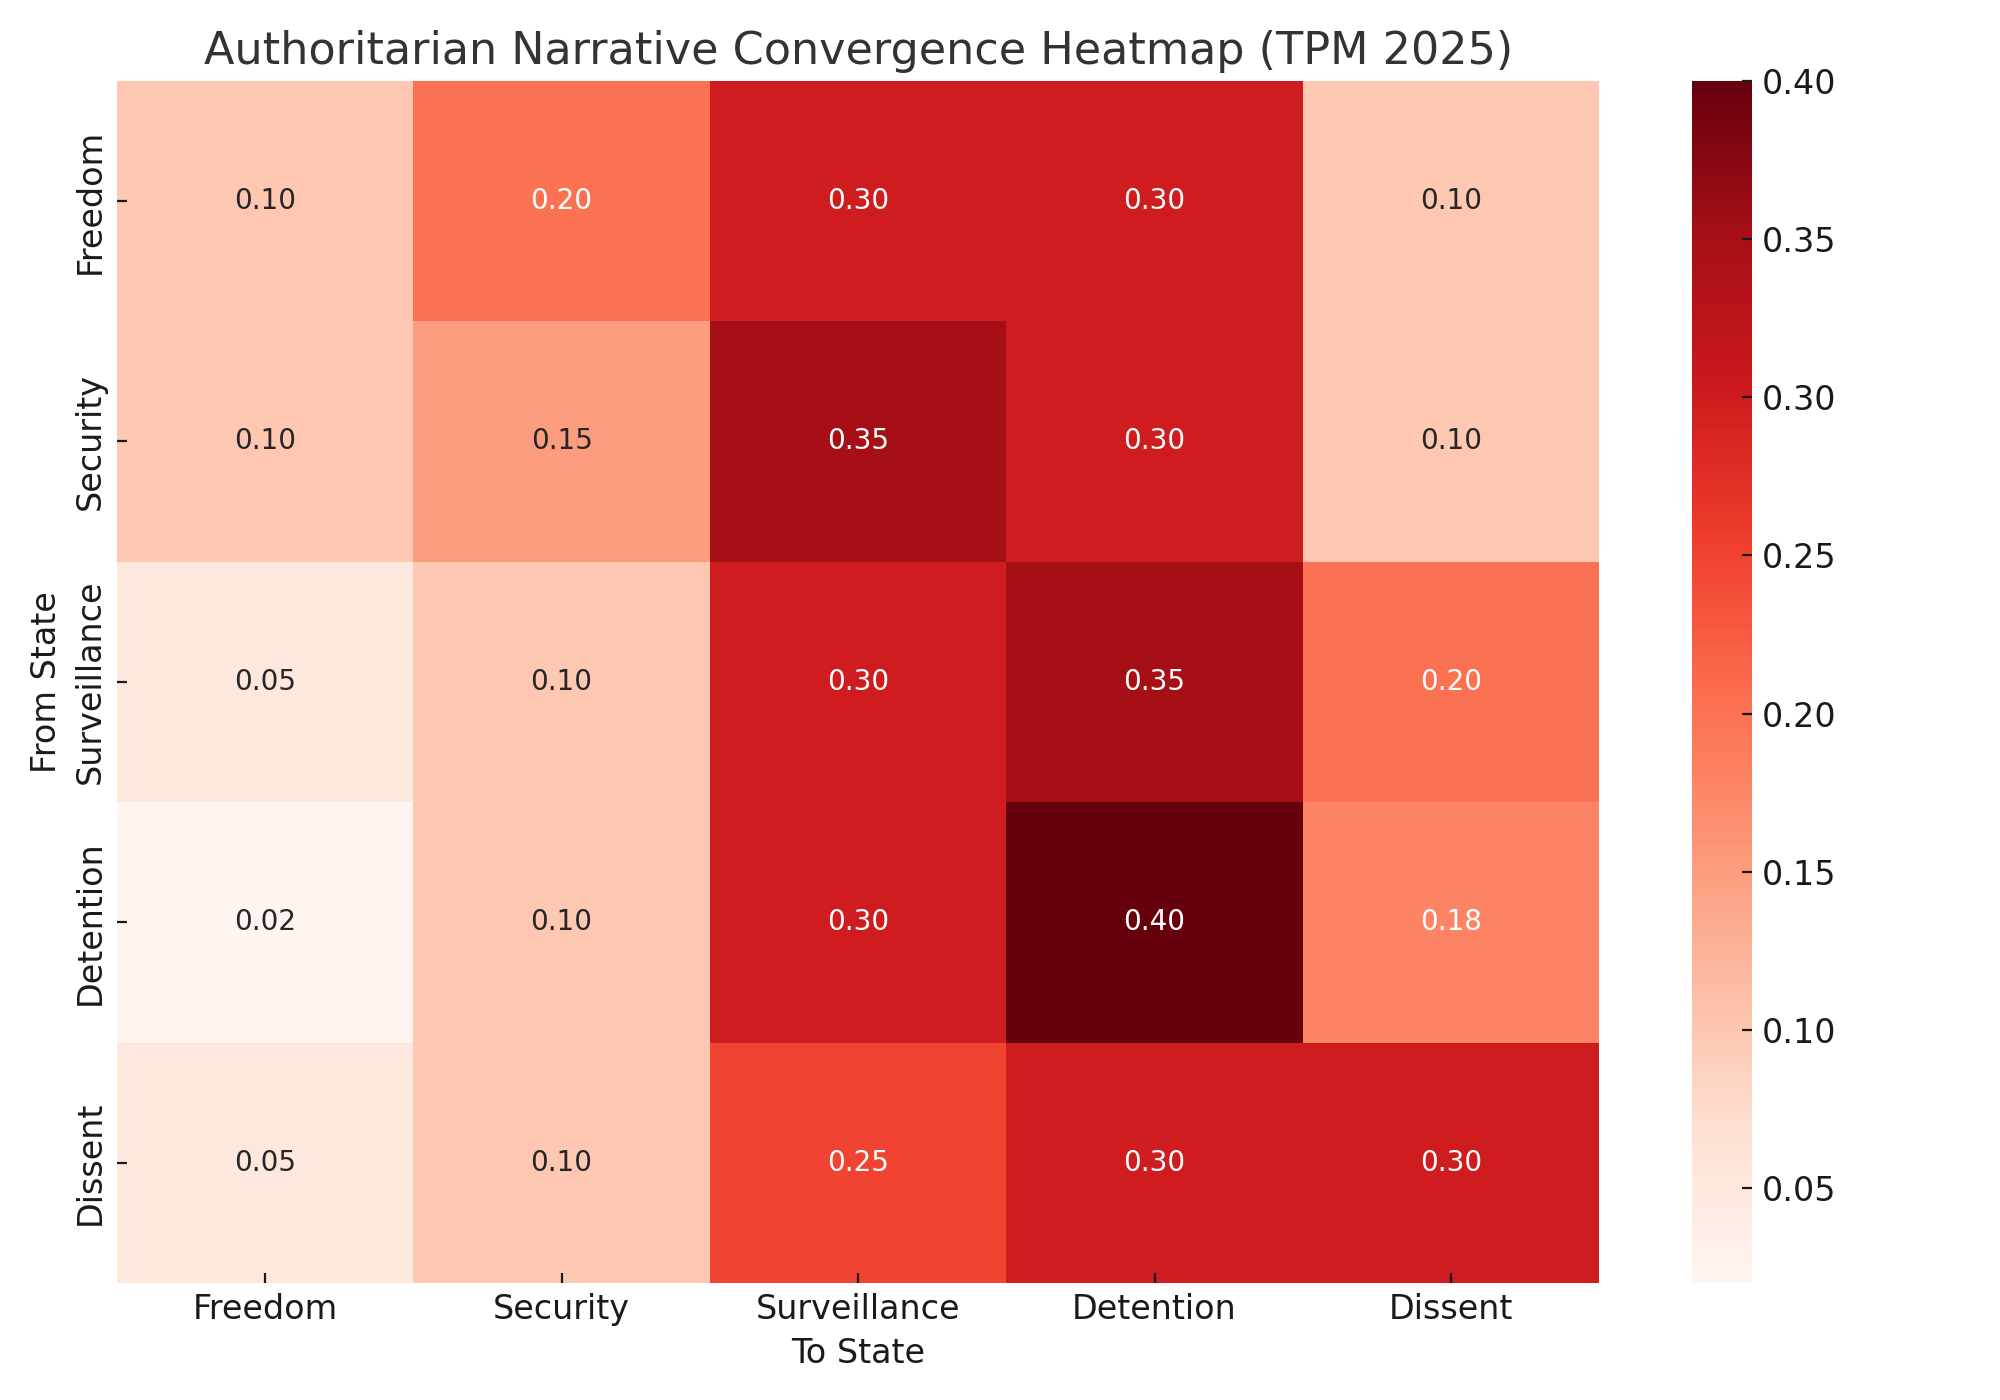
\includegraphics[width=0.9\textwidth]{figures/tpm_drift_palantir.png}
  \caption{Dripping TPM entropy heatmap illustrating authoritarian narrative convergence in DHS policy via Palantir}
\end{figure}

\section*{Conclusion: A Government Forgotten, Remembered by Algorithms}
What we are witnessing is not merely privatization. It is the outsourcing of state memory to opaque platforms. Democracy depends on collective recall, civic documentation, and transparent jurisprudence. When memory becomes proprietary, the algorithm owns history—and decides what you can know.

\begin{flushright}
\textit{--- Ronald J. Botelho, 2025}
\end{flushright}

\newpage

\chapter{Chapter 1: Foundations of Collapse}
\section*{The Architecture of Erosion}
It doesn’t begin with a coup. It begins with permission. The slow recalibration of what is acceptable, expected, and ultimately normalized. Collapse is less about a system’s destruction than about its redefinition.

In this chapter, we explore the mechanisms by which entropy creeps into public discourse, institutions, and civic behavior. By treating disinformation not just as deception but as a thermodynamic transaction—an entropic tax on cognition—we identify how each falsehood compounds institutional decay.

Modern autocracy rarely announces itself. It leaks in through Supreme Court decisions, data pipelines, and performative patriotism. This book is a chronicle of those leaks—and the tipping points they produce.

\newpage

\chapter{Chapter 2: Elon Musk and the Infrastructure of Digital Autocracy}
\section*{Introduction: Silicon Influence and the Subversion of Public Space}
Before the era of Rufo, Vance, or Cruz, there was William F. Buckley Jr., a conservative provocateur whose 1951 book \textit{God and Man at Yale} framed universities as ideological battlegrounds. Buckley’s legacy is not simply polemical—it is structural. He embedded the idea that the academy was both enemy and opportunity. That to seize the future, one had to reprogram the university.

In today's ecosystem, Buckley's template has been digitized and militarized. Platforms controlled by figures like Elon Musk—infused with AI, surveillance capitalism, and opaque algorithms—extend Buckley’s ideological warfare into the infrastructure of digital life. Universities, once shaped by editorial columns and political lectures, are now shaped by code, content throttling, and targeted disinformation.

The privatized systems of Musk’s empire (including SpaceX contracts with DHS, X/Twitter’s role in shaping political discourse, and Neuralink’s transhumanist ambitions) act as contemporary expressions of Buckley’s logic—radical conservatism disguised as innovation, censorship framed as freedom.

As we move through this chapter, we trace the evolution from Buckley’s patrician critiques to Musk’s techno-authoritarian reach. It is a lineage, not an aberration.

% (To be continued with full chapter narrative and figures)
